% Created 2016-04-21 Do 11:51
\documentclass[a4paper, captions=tableheading]{tufte-book}
        \usepackage[utf8]{inputenc}
\usepackage[ngerman, english]{babel}
\usepackage[T1]{fontenc}
\usepackage{footnote}
\usepackage{minitoc}
\usepackage{booktabs}
\usepackage{longtable}
\usepackage{lmodern}
\usepackage{graphicx}
\usepackage{hyperref}
\usepackage{url}
\usepackage{fancyvrb}
\usepackage{color}
\usepackage{xcolor}
\usepackage{amsmath}
\usepackage{amssymb}
\usepackage{array}
\usepackage{listings}
\usepackage{rotating}
\usepackage{multicol}
\usepackage{pdflscape}
\usepackage{ctable}
\usepackage{parskip}
\usepackage{anysize}
\usepackage{supertabular}
\usepackage{minted}
\usepackage{natbib}
\usemintedstyle{perldoc}
\usepackage{gensymb}
\usepackage{nicefrac}
\usepackage{units}
\usepackage{marginfix}
\usepackage{breakurl}
\usepackage{float}
\usepackage{placeins}
\usepackage{tabu}
\usepackage{tabulary}
\usepackage{tocloft}
\usepackage{titlesec}
\newcommand{\sectionbreak}{\clearpage}
\makeatletter
\renewcommand{\@tufte@reset@par}{\setlength{\RaggedRightParindent}{0pt}\setlength{\JustifyingParindent}{0pt}\setlength{\parindent}{0pt}\setlength{\parskip}{0.5\baselineskip}}
\@tufte@reset@par
\renewcommand{\@tufte@margin@par}{\setlength{\RaggedRightParindent}{0pt}\setlength{\JustifyingParindent}{0pt}\setlength{\parindent}{0pt}\setlength{\parskip}{0.5\baselineskip}}
\makeatother
\geometry{left=20mm, textwidth=130mm, marginparsep=8mm, marginparwidth=40mm}
\definecolor{darkblue}{rgb}{0,0,.5}
\definecolor{darkgreen}{rgb}{0,.5,0}
\definecolor{islamicgreen}{rgb}{0.0, 0.56, 0.0}
\definecolor{darkred}{rgb}{0.5,0,0}
\definecolor{mintedbg}{rgb}{0.95,0.95,0.95}
\definecolor{arsenic}{rgb}{0.23, 0.27, 0.29}
\definecolor{prussianblue}{rgb}{0.0, 0.19, 0.33}
\definecolor{coolblack}{rgb}{0.0, 0.18, 0.39}
\definecolor{cobalt}{rgb}{0.0, 0.28, 0.67}
\definecolor{moonstoneblue}{rgb}{0.45, 0.66, 0.76}
\definecolor{aliceblue}{rgb}{0.94, 0.97, 1.0}
\hypersetup{colorlinks=true, breaklinks=true, linkcolor=coolblack, anchorcolor=blue, citecolor=islamicgreen, filecolor=blue,  menucolor=blue,  urlcolor=violet}
\renewcommand\thefootnote{\textcolor{darkred}{\arabic{footnote}}}
\renewcommand{\theFancyVerbLine}{\sffamily\textcolor[rgb]{0.7,0.7,0.7}{\tiny\arabic{FancyVerbLine}}}
\setcounter{secnumdepth}{3}
\titleformat{\section}{\normalfont\Large\itshape\color{black}} {\llap{\colorbox{coolblack}{\parbox{1.5cm}{\hfill\color{white}\thesection}}}}{1em}{}[]
\titleformat{\subsection}{\normalfont\large\itshape\color{black}} {\llap{\colorbox{aliceblue}{\parbox{1.5cm}{\hfill\color{coolblack}\thesubsection}}}}{1em}{}[]
\titleformat{\subsubsection}{\normalfont\large\itshape\color{black}} {\llap{\colorbox{aliceblue}{\parbox{1.5cm}{\hfill\color{coolblack}\thesubsubsection}}}}{1em}{}[]
\setcounter{secnumdepth}{3}
\author{Göran Kirchner}
\date{\today}
\title{Notes on R}
\hypersetup{
 pdfauthor={Göran Kirchner},
 pdftitle={Notes on R},
 pdfkeywords={},
 pdfsubject={},
 pdfcreator={Emacs 24.5.1 (Org mode 8.3.1)},
 pdflang={English}}
\begin{document}

\maketitle

\chapter{Packages}
\label{sec:orgheadline1}

\chapter{Data}
\label{sec:orgheadline2}

\begin{minted}[bgcolor=mintedbg,frame=none,framesep=0pt,mathescape=true,fontsize=\footnotesize,gobble=0]{r}
head(movies)
\end{minted}

\begin{center}
\begin{tabular}{lrlrrrll}
\toprule
Title & Year & Rating & Runtime & Critic.Score & Box.Office & Awards & International\\
\midrule
The Whole Nine Yards & 2000 & R & 98 & 45 & 57.3 & FALSE & FALSE\\
Cirque du Soleil: Journey of Man & 2000 & G & 39 & 45 & 13.4 & TRUE & FALSE\\
Gladiator & 2000 & R & 155 & 76 & 187.3 & TRUE & TRUE\\
Dinosaur & 2000 & PG & 82 & 65 & 135.6 & TRUE & FALSE\\
Big Momma's House & 2000 & PG-13 & 99 & 30 & 0.5 & TRUE & TRUE\\
Gone in Sixty Seconds & 2000 & PG-13 & 118 & 24 & 101 & TRUE & FALSE\\
\bottomrule
\end{tabular}
\end{center}

\chapter{Simple Visualization}
\label{sec:orgheadline14}


\section{One Categorical Variable}
\label{sec:orgheadline6}

\subsection{base}
\label{sec:orgheadline3}

\begin{minted}[bgcolor=mintedbg,frame=none,framesep=0pt,mathescape=true,fontsize=\footnotesize,gobble=0]{r}
plot(
	x = movies$Rating,
	main = "Count of Movies by Rating",
	xlab = "Rating",
	ylab = "Count of Movies")
\end{minted}

\includegraphics[height=6cm]{img/1-cat-base-01.png}


\begin{minted}[bgcolor=mintedbg,frame=none,framesep=0pt,mathescape=true,fontsize=\footnotesize,gobble=0]{r}
dotchart(
	x = table(movies$Rating),
	pch = 16,
	main = "Count of Movies by Rating",
	xlab = "Count of Movies",
	ylab = "Rating")
\end{minted}

\includegraphics[height=6cm]{img/1-cat-base-02.png}


\begin{minted}[bgcolor=mintedbg,frame=none,framesep=0pt,mathescape=true,fontsize=\footnotesize,gobble=0]{r}
pie(
	x = table(movies$Awards),
	clockwise = TRUE,
	main = "Proportion of Movies that Won Awards")
\end{minted}

\includegraphics[height=6cm]{img/1-cat-base-03.png}

\subsection{lattice}
\label{sec:orgheadline4}

\begin{minted}[bgcolor=mintedbg,frame=none,framesep=0pt,mathescape=true,fontsize=\footnotesize,gobble=0]{r}
library(lattice)
# Create frequency table of ratings
movies <- read.csv("data/movies.csv")
table <- table(movies$Rating)
ratings <- as.data.frame(table)
names(ratings)[1] <- "Rating"
names(ratings)[2] <- "Count"
print(ratings)
\end{minted}

\begin{center}
\begin{tabular}{lr}
\toprule
Rating & Count\\
\midrule
G & 93\\
PG & 497\\
PG-13 & 1225\\
R & 1423\\
\bottomrule
\end{tabular}
\end{center}

\begin{minted}[bgcolor=mintedbg,frame=none,framesep=0pt,mathescape=true,fontsize=\footnotesize,gobble=0]{r}
library(lattice)
# Create frequency table of ratings
movies <- read.csv("data/movies.csv")
table <- table(movies$Rating)
ratings <- as.data.frame(table)
names(ratings)[1] <- "Rating"
names(ratings)[2] <- "Count"
barchart(
	x = Count ~ Rating,
	data = ratings,
	main = "Count of Movies by Rating",
	xlab = "Rating")
\end{minted}

\includegraphics[height=6cm]{img/1-cat-lattice-01.png}

\begin{minted}[bgcolor=mintedbg,frame=none,framesep=0pt,mathescape=true,fontsize=\footnotesize,gobble=0]{r}
library(lattice)
# Create frequency table of ratings
movies <- read.csv("data/movies.csv")
table <- table(movies$Rating)
ratings <- as.data.frame(table)
names(ratings)[1] <- "Rating"
names(ratings)[2] <- "Count"
dotplot(
	x = Rating ~ Count,
	data = ratings,
	main = "Count of Movies by Rating",
	ylab = "Rating")
\end{minted}

\includegraphics[height=6cm]{img/1-cat-lattice-02.png}

\begin{minted}[bgcolor=mintedbg,frame=none,framesep=0pt,mathescape=true,fontsize=\footnotesize,gobble=0]{r}
library(lattice)
# Create frequency table of ratings
movies <- read.csv("data/movies.csv")
table <- table(movies$Rating)
ratings <- as.data.frame(table)
names(ratings)[1] <- "Rating"
names(ratings)[2] <- "Count"
histogram(
	x = ~Rating,
	data = movies,
	main = "Percent of Movies by Rating")
\end{minted}

\includegraphics[height=6cm]{img/1-cat-lattice-03.png}

\subsection{ggplot2}
\label{sec:orgheadline5}

\begin{minted}[bgcolor=mintedbg,frame=none,framesep=0pt,mathescape=true,fontsize=\footnotesize,gobble=0]{r}
library(ggplot2)
movies <- read.csv("data/movies.csv")
ggplot(
		data = movies,
		aes(x = Rating)) +
		geom_bar() +
		ggtitle("Count of Movies by Rating")
\end{minted}

\includegraphics[height=6cm]{img/1-cat-ggplot2-01.png}

\begin{minted}[bgcolor=mintedbg,frame=none,framesep=0pt,mathescape=true,fontsize=\footnotesize,gobble=0]{r}
library(ggplot2)
library(lattice)
# Create frequency table of ratings
movies <- read.csv("data/movies.csv")
table <- table(movies$Rating)
ratings <- as.data.frame(table)
names(ratings)[1] <- "Rating"
names(ratings)[2] <- "Count"
ggplot(
	data = ratings,
	aes(x = Rating, y = Count)) +
	geom_point() +
	coord_flip() +
	ggtitle("Count of Movies by Rating")
\end{minted}

\includegraphics[height=6cm]{img/1-cat-ggplot2-02.png}

\begin{minted}[bgcolor=mintedbg,frame=none,framesep=0pt,mathescape=true,fontsize=\footnotesize,gobble=0]{r}
library(ggplot2)
movies <- read.csv("data/movies.csv")
ggplot(
	data = movies,
	aes(x = "", fill = Awards)) +
	geom_bar() +
	coord_polar(theta = "y") +
	ggtitle("Proportion of Movies that Won Awards") +
	ylab("")
\end{minted}

\includegraphics[height=6cm]{img/1-cat-ggplot2-03.png}

\section{One Numeric Variable}
\label{sec:orgheadline10}

\subsection{base}
\label{sec:orgheadline7}

\begin{minted}[bgcolor=mintedbg,frame=none,framesep=0pt,mathescape=true,fontsize=\footnotesize,gobble=0]{r}
movies <- read.csv("data/movies.csv")
plot(
		x = movies$Runtime,
		y = jitter(rep(0, nrow(movies))),
		main = "Distribution of Movie Runtimes",
		xlab = "Runtime (minutes)",
		ylab = "",
		yaxt = "n",
		pch = 16,
		col = rgb(0, 0, 0.3, 0.2))
\end{minted}

\includegraphics[height=6cm]{img/1-num-base-01.png}

\begin{minted}[bgcolor=mintedbg,frame=none,framesep=0pt,mathescape=true,fontsize=\footnotesize,gobble=0]{r}
movies <- read.csv("data/movies.csv")
boxplot(
		x = movies$Runtime,
		horizontal = TRUE,
		main = "Distribution of Movie Runtimes",
		xlab = "Runtime (minutes)")
\end{minted}

\includegraphics[height=6cm]{img/1-num-base-02.png}

\begin{minted}[bgcolor=mintedbg,frame=none,framesep=0pt,mathescape=true,fontsize=\footnotesize,gobble=0]{r}
movies <- read.csv("data/movies.csv")
hist(
		x = movies$Runtime,
		breaks = 30,
		main = "Distribution of Movie Runtimes",
		xlab = "Runtime (minutes)")
\end{minted}

\includegraphics[height=6cm]{img/1-num-base-03.png}

\begin{minted}[bgcolor=mintedbg,frame=none,framesep=0pt,mathescape=true,fontsize=\footnotesize,gobble=0]{r}
movies <- read.csv("data/movies.csv")
plot(
		x = density(movies$Runtime),
		main = "Distribution of Movie Runtimes",
		xlab = "Runtime (minutes)")
\end{minted}

\includegraphics[height=6cm]{img/1-num-base-04.png}

\subsection{lattice}
\label{sec:orgheadline8}

\begin{minted}[bgcolor=mintedbg,frame=none,framesep=0pt,mathescape=true,fontsize=\footnotesize,gobble=0]{r}
movies <- read.csv("data/movies.csv")
library(lattice)
bwplot(
		x = ~Runtime,
		data = movies,
		main = "Distribution of Movie Runtimes",
		xlab = "Runtime (minutes)")
\end{minted}

\includegraphics[height=6cm]{img/1-num-lattice-02.png}

\begin{minted}[bgcolor=mintedbg,frame=none,framesep=0pt,mathescape=true,fontsize=\footnotesize,gobble=0]{r}
movies <- read.csv("data/movies.csv")
library(lattice)
histogram(
		x = ~Runtime,
		data = movies,
		main = "Distribution of Movie Runtimes",
		xlab = "Runtime (minutes)")
\end{minted}

\includegraphics[height=6cm]{img/1-num-lattice-03.png}

\begin{minted}[bgcolor=mintedbg,frame=none,framesep=0pt,mathescape=true,fontsize=\footnotesize,gobble=0]{r}
movies <- read.csv("data/movies.csv")
library(lattice)
densityplot(
		x = ~Runtime,
		data = movies,
		main = "Distribution of Movie Runtimes",
		xlab = "Runtime (minutes)")
\end{minted}

\includegraphics[height=6cm]{img/1-num-lattice-04.png}

\subsection{ggplot2}
\label{sec:orgheadline9}

\begin{minted}[bgcolor=mintedbg,frame=none,framesep=0pt,mathescape=true,fontsize=\footnotesize,gobble=0]{r}
library(ggplot2)
movies <- read.csv("data/movies.csv")
ggplot(
		data = movies,
		aes(x = Runtime, stat = "count")) +
		geom_dotplot(
				binwidth = 1,
				stackdir = "center") +
		ggtitle("Distribution of Movie Runtimes") +
		xlab("Runtime (minutes)")
\end{minted}

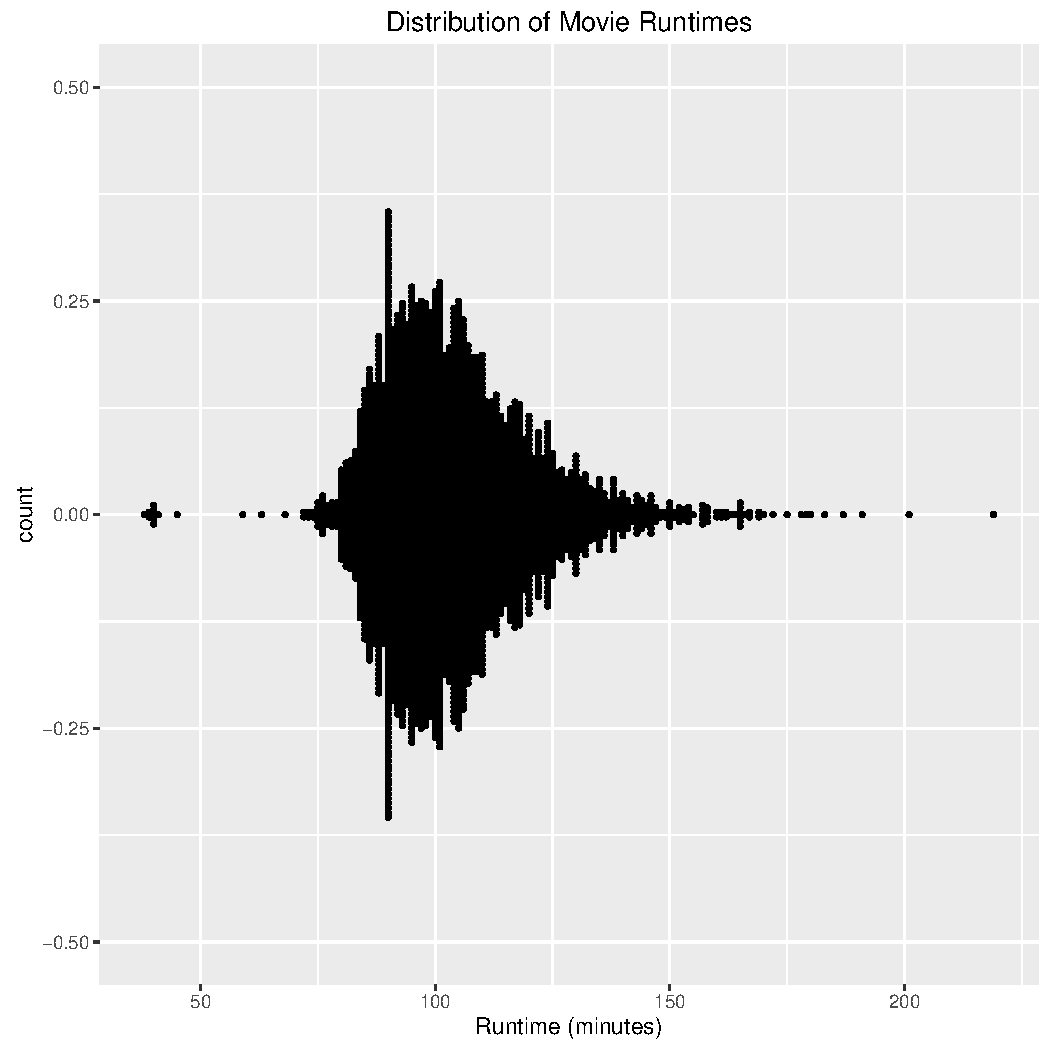
\includegraphics[height=6cm]{img/1-num-ggplot2-01.png}


\begin{minted}[bgcolor=mintedbg,frame=none,framesep=0pt,mathescape=true,fontsize=\footnotesize,gobble=0]{r}
library(ggplot2)
movies <- read.csv("data/movies.csv")
ggplot(
		data = movies,
		aes(x = Runtime, y = Runtime)) +
		geom_boxplot() +
		coord_flip() +
		ggtitle("Distribution of Movie Runtimes") +
		xlab("") +
		ylab("Runtime (minutes)") +
		theme(
				axis.text.y = element_blank(),
				axis.ticks.y = element_blank())
\end{minted}

\includegraphics[height=6cm]{img/1-num-ggplot2-02.png}


\begin{minted}[bgcolor=mintedbg,frame=none,framesep=0pt,mathescape=true,fontsize=\footnotesize,gobble=0]{r}
library(ggplot2)
movies <- read.csv("data/movies.csv")
ggplot(
		data = movies,
		aes(x = Runtime)) +
		geom_histogram(binwidth = 10) +
		ggtitle("Distribution of Movie Runtimes") +
		xlab("Runtime (minutes)")
\end{minted}

\includegraphics[height=6cm]{img/1-num-ggplot2-03.png}


\begin{minted}[bgcolor=mintedbg,frame=none,framesep=0pt,mathescape=true,fontsize=\footnotesize,gobble=0]{r}
library(ggplot2)
movies <- read.csv("data/movies.csv")
ggplot(
		data = movies,
		aes(x = Runtime)) +
		geom_density() +
		ggtitle("Distribution of Movie Runtimes") +
		xlab("Runtime (minutes)")
\end{minted}

\includegraphics[height=6cm]{img/1-num-ggplot2-04.png}

\section{Two Categorical Variables}
\label{sec:orgheadline11}

\section{Two Numeric Variables}
\label{sec:orgheadline12}

\section{Both a Categorical and a Numeric Variable}
\label{sec:orgheadline13}

\chapter{Intermediate Visualization}
\label{sec:orgheadline16}

\section{Radar Plot}
\label{sec:orgheadline15}

\begin{table}\footnotesize
\caption{\label{tab:orgtable1}
Some Values}
\centering
\begin{tabular}{lrrr}
\toprule
Category & Val1 & Val2 & Val3\\
\midrule
A & 2 & 3 & 4\\
B & 2 & 2 & 2\\
C & 4 & 1 & 2\\
D & 3 & 1 & 3\\
E & 3 & 2 & 2\\
F & 2 & 4 & 3\\
\bottomrule
\end{tabular}
\end{table}

\begin{minted}[bgcolor=mintedbg,frame=none,framesep=0pt,mathescape=true,fontsize=\footnotesize,gobble=0]{r}
coord_radar <- function (theta = "x", start = 0, direction = 1)
{
		theta <- match.arg(theta, c("x", "y"))
		r <- if (theta == "x")
				"y"
		else "x"
		ggproto("CordRadar", CoordPolar, theta = theta, r = r, start = start,
				direction = sign(direction),
				is_linear = function(coord) TRUE)
}
\end{minted}


\begin{minted}[bgcolor=mintedbg,frame=none,framesep=0pt,mathescape=true,fontsize=\footnotesize,gobble=0]{r}
ggplot(xs, aes(x=V, y=H, color=Category, group=Category, fill=Category)) +
geom_polygon(alpha=.1) +
coord_radar() +
ggtitle("Radar Plot") +
xlab("V*") + ylab("Hight")
\end{minted}

\includegraphics[width=.9\linewidth]{img/radar-01.png}

\chapter{Advanced Visualization}
\label{sec:orgheadline17}



\chapter{Quellen}
\label{sec:orgheadline20}

\section{General}
\label{sec:orgheadline18}

\begin{itemize}
\item \url{http://www.cookbook-r.com/}
\item \url{http://www.datendesign-r.de/beispiele/}
\item \url{https://www.rstudio.com/resources/cheatsheets/}
\end{itemize}


\section{Special}
\label{sec:orgheadline19}

\begin{itemize}
\item \url{http://stackoverflow.com/questions/22064611/how-to-draw-rotated-axes-in-r}
\end{itemize}
\end{document}